\chapter{LITERATURE REVIEW}

\section{Vision-Language model}
In the past few years, many works have shown the ability to utilize textual information with the image task by training with image text pair, such as Contrastive Language-Image Pre-training (CLIP) \shortcite{radford2021learning}, \textbf{A} \textbf{L}arge-scale \textbf{I}ma\textbf{G}e and \textbf{N}oisy-text embedding (ALIGN) \shortcite{jia2021scaling}.
By training with a large amount of the image-text pair dataset, the ALIGN model could make up for the noisy image description and surpass the model, which was trained with the benchmark dataset in the zero shot image classification task.
Recently \textbf{Co}ntrastive \textbf{Ca}ptioner (CoCa) \shortcite{yu2022coca} proposed a vision-language encoder-decoder model which was trained with image-text contrastive loss and captioning loss
Cross attention layers were added to join image-text modality.
The CoCa model performed linear probing image classification on ImageNet with top-1\% 90.6\% accuracy.
In this research, we adopted the two stream encoder method same as CLIP, and we also used a cross attention layer to create image-text representation for classification.
% \textcolor{red}{todo: Add detail about blip model}

\begin{figure}[h]
    \caption{CLIP Classification example}
    \label{fig:clip_classification}
    \centering
    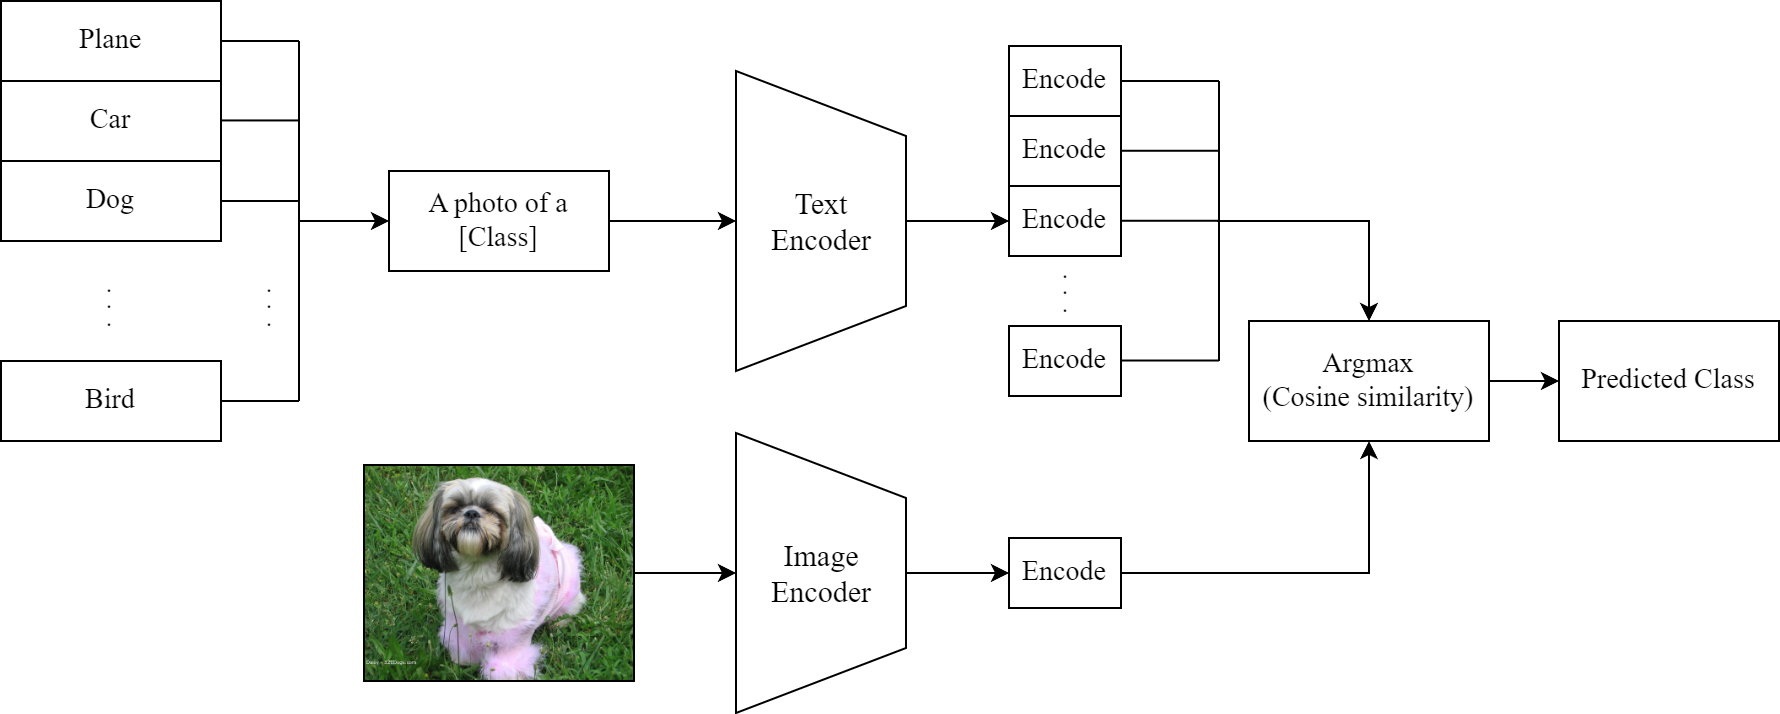
\includegraphics[width=1\textwidth]{Images/CLIPClassification.png}
    \small
\end{figure}

\section{Knowledge Distillation and Self-Distillation}
Knowledge Distillation was firstly proposed by \shortciteA{geoffrey2014distilling} to compress the model size while maintaining the model performance as much as possible.
The method contained a smaller student model and a single or multiple larger teacher model.
The knowledge was transferred by optimizing the student model output to match the teacher's output.
\shortciteA{furlanello2018born} investigated knowledge distillation using a student model size the same as the teacher model, showing improvement in the student model.
Such a method is called self-distillation.
The self-distillation has widely adopted in semi-supervised image classification tasks, such as Mean Teacher \shortcite{tarvainen2017mean}, EMAN \shortcite{cai2021exponential} and FixMatch \shortcite{sohn2020fixmatch}.
DINO \shortciteA{caron2021emerging} proposed self-distillation pre-training without using any label, which resulted in performance improvement.
In this paper, we extended the self-distillation by creating representation which was image-text combined representation, and we trained the student model to match teacher softmax outputs.

% \section{Semi-Supervised Learning}
% In semi-supervised learning, recent method can be divided into two category, pseudo-labeling and consistency-based. The consistency-based \shortcite{laine2016temporal, tarvainen2017mean, xie2020unsupervised, verma2022interpolation} is focus on training two models by giving same image with difference augmentation, and those two model are train to output very similar probability output using consistency loss. $\Pi$-Model and Temporal Ensemble \shortcite{laine2016temporal} training with consistency loss and adding noise to model weights using dropout. UDA \shortcite{xie2020unsupervised} apply weak and strong image augmentation to train two models simultaneously. On the other  hand, pseudo-labeling \shortcite{sohn2020fixmatch, cai2022semisupervised, pham2021meta} focus on assign label to the unlabeled images by pre-train a teacher model with labeled images. This work is fall into consistency-based group, training with the logits output of the teacher model directly.

% \section{Image Captioning}


% \begin{table}[]
% \begin{tabular}{lllllll}
% Model & Param & Key Contribution                                                            & ImageNet1\%  Top1\% & ImageNet10\% Top1\% &   &   \\
% Semi-ViT/Base 2022 & 86M       & Using Teacher-Student and propose Batch MixUp to mix label and unlabel image & 71.0                & 79.7                &   &   \\
% Semi-ViT/Large     & 307M      &                                                                              & 77.3                & 83.3                &   &   \\
% FixMatch 2020      & ResNet-50 & Propose strong and weak augmentation using consistency regularization        &                     & 71.46               &   &   \\
%                    &           &                                                                              &                     &                     &   &
% \end{tabular}
% \end{table}